\subsection{Labyrinth}

The final experimental setting for progressive networks is Labyrinth,
a 3D maze environment where the inputs are rendered images granting partial
observability and the agent outputs discrete actions,
including looking up, down, left, or right and moving forward,
backwards, left, or right. The tasks as well as the level maps are
diverse and involve getting positive scores for `eating' good items
(apples, strawberries) and negative scores for eating bad items
(mushrooms, lemons). Details can be found in the appendix. While there is conceptual and
visual overlap between the different tasks, the tasks present a
challenging set of diverse game elements (Figure
\ref{fig:datasets}).

\begin{figure}[h]
  \centering
    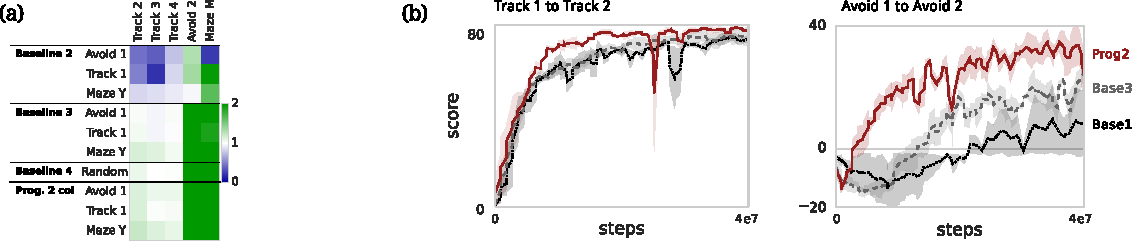
\includegraphics[width=\textwidth]{figures/transfer_lab.pdf}
    \caption{Transfer scores and example learning curves for Labyrinth tasks. Colours indicate transfer (clipped at 2). The learning curves show two examples of two-column progressive performance vs. baselines 1 and 3.}
    \label{fig:lab}
\end{figure}

As in the other domains, the progressive approach yields more positive transfer than any of the baselines (see Fig.~\ref{fig:lab}a and Table~\ref{table:main}). We observe less transfer on the Seek Track levels, which have dense reward items throughout the maze and are easily learned. Note that even for these easy cases, baseline 2 shows negative transfer because it cannot learn new low-level visual features, which are important because the reward items change from task to task. The learning curves in Fig.~\ref{fig:lab}b exemplify the typical results seen in this domain: on simpler games, such as Track 1 and 2, learning is rapid and stable by all agents. On more difficult games, with more complex game structure, the baselines struggle and progressive nets have an advantage.
